% Editable vector schematic. Spans have equal widths for layout, not token counts.
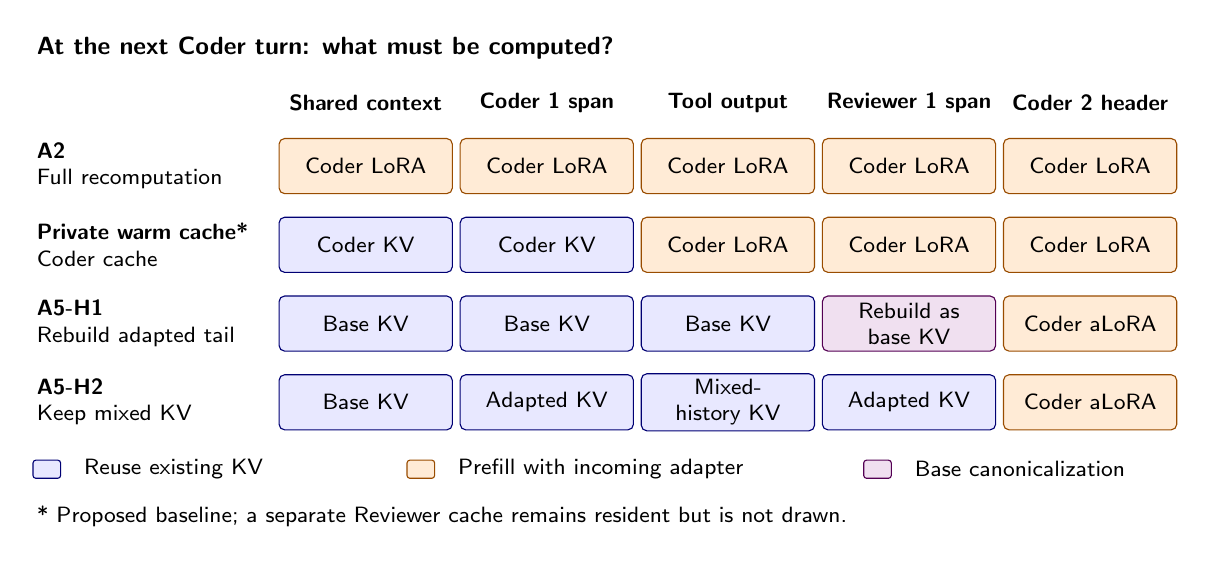
\begin{tikzpicture}[
  x=1cm,y=1cm,font=\sffamily\footnotesize,
  box/.style={draw,rounded corners=2pt,minimum width=2.2cm,
    minimum height=.70cm,text width=2.04cm,align=center,inner sep=2pt},
  swatch/.style={draw,rounded corners=1pt,minimum width=.35cm,
    minimum height=.23cm,inner sep=0pt},
  reuse/.style={box,draw=blue!45!black,fill=blue!9},
  work/.style={box,draw=orange!60!black,fill=orange!16},
  canon/.style={box,draw=violet!65!black,fill=violet!12}
]
\node[anchor=west,font=\sffamily\small\bfseries] at (0,.95)
  {At the next Coder turn: what must be computed?};
\foreach \x/\name in {4.3/Shared context,6.6/Coder 1 span,
  8.9/Tool output,11.2/Reviewer 1 span,13.5/Coder 2 header}
  \node[align=center,font=\sffamily\footnotesize\bfseries] at (\x,.25) {\name};

\node[anchor=west,align=left,text width=2.8cm] at (0,-.55)
  {\textbf{A2}\\Full recomputation};
\foreach \x in {4.3,6.6,8.9,11.2,13.5}
  \node[work] at (\x,-.55) {Coder LoRA};

\node[anchor=west,align=left,text width=2.8cm] at (0,-1.55)
  {\textbf{Private warm cache*}\\Coder cache};
\foreach \x in {4.3,6.6}
  \node[reuse] at (\x,-1.55) {Coder KV};
\foreach \x in {8.9,11.2,13.5}
  \node[work] at (\x,-1.55) {Coder LoRA};

\node[anchor=west,align=left,text width=2.8cm] at (0,-2.55)
  {\textbf{A5-H1}\\Rebuild adapted tail};
\foreach \x in {4.3,6.6,8.9}
  \node[reuse] at (\x,-2.55) {Base KV};
\node[canon] at (11.2,-2.55) {Rebuild as\\base KV};
\node[work] at (13.5,-2.55) {Coder aLoRA};

\node[anchor=west,align=left,text width=2.8cm] at (0,-3.55)
  {\textbf{A5-H2}\\Keep mixed KV};
\node[reuse] at (4.3,-3.55) {Base KV};
\node[reuse] at (6.6,-3.55) {Adapted KV};
\node[reuse] at (8.9,-3.55) {Mixed-history KV};
\node[reuse] at (11.2,-3.55) {Adapted KV};
\node[work] at (13.5,-3.55) {Coder aLoRA};

\node[swatch,draw=blue!45!black,fill=blue!9] at (.25,-4.4) {};
\node[anchor=west] at (.6,-4.4) {Reuse existing KV};
\node[swatch,draw=orange!60!black,fill=orange!16] at (5.0,-4.4) {};
\node[anchor=west] at (5.35,-4.4) {Prefill with incoming adapter};
\node[swatch,draw=violet!65!black,fill=violet!12] at (10.8,-4.4) {};
\node[anchor=west] at (11.15,-4.4) {Base canonicalization};
\node[anchor=west,align=left,text width=14.6cm,font=\sffamily\footnotesize]
  at (0,-5.0) {* Proposed baseline; a separate Reviewer cache remains resident but is not drawn.};
\end{tikzpicture}
